\newSec[PrincSOLID]{SOLID}{2}

\newSec[PrincSOLIDSingle]{Single Responsibility Principle}{3}
Jeder Klasse des zugrundeliegenden Codes kann eine definierte und subjketiv kleine Aufgabe zugewiesen werden. Als Beispiel soll die nachfolgende Beschreibung dienen.

Beispiel \CodeClass{Input}:\\
Die Aufgabe dieser Klasse ist es, einen Wert vom Typ \CodeClass{Value} für eine weitere Bearbeitung bereitzustellen.\\
\begin{itemize}
\item Implementiert \CodeMeth{getInputUnit()} aus \CodeClass{Inputable}.
\item Erlaubt das Zuweisen eines Objekt-Pointers vom Typ \CodeClass{Outputable}, von welchem Daten abgefragt werden können.
\item Gibt den zugewiesenen \CodeClass{Outputable}-Pointer zurück (\CodeMeth{getInputAddr}).
\end{itemize}


\href{https://github.com/MobMonRob/ROSLabDrohne/blob/979c6057922852eac0af20a52e29393d41adfee5/Code/Controller/include/Controller/Input.h}{Link: Controller/Input.h}


Neben der genannten semantischen Einschätzung des zugrundeliegenden Codes soll an dieser Stelle folgendes Theorem eingeführt werden:

\newSec[PrincGRASPKoppNew]{Maag-Uhlmann-Theorem}{4}
Grundsätzlich kann ein Projekt mit der Menge an Objekten des Domänenmodells umgesetzt werden. Je höher das Verhältnis $q =\frac{used ClassCount Project + used Extern Packages}{ObjectCount Domain Model}$, desto eher ist eine feingranularere Aufgabenverteilung an die jeweiligen Klassen zu erwarten. Ein Wert $q=1$ entspricht der Umsetzung aller Funktionalität innerhalb der Objekte (dann Klassen) des Domänenmodells, hiervon ist abzuraten.
In unserem Projekt befinden sich 37 eingesetzte Klassen und Pakete, entgegen stehen 8 Objekte im Domänenmodell. Hieraus folgt: $q = 4.625$.



\newSec[PrincSOLIDOC]{Open/Closed Principle}{3}
Beispiel (siehe \refImg{fig:OC}): \CodeClass{SafetyProvider} und \CodeClass{SafetyRequirement}\\
Die Klasse \CodeClass{SafetyProvider} soll sicherstellen, dass der Flug der Drohne sicher durchgeführt werden kann. Hierzu werden verschiedene Anforderungen (\CodeClass{SafetyProvider}) hinzugefügt. Bei der \CodeClass{SafetyProvider} handelt es sich um eine \textit{full virtual} Klasse\footnotemark{1}. Hiervon werden die tatsächlichen Anforderungen abgeleitet.

\href{https://github.com/MobMonRob/ROSLabDrohne/blob/979c6057922852eac0af20a52e29393d41adfee5/Code/Domain/include/Domain/SafetyProvider.h}{Link: Domain/SafetyProvider.h}\\
\href{https://github.com/MobMonRob/ROSLabDrohne/blob/979c6057922852eac0af20a52e29393d41adfee5/Code/Domain/src/SafetyProvider.cpp}{Link: Domain/SafetyProvider.cpp}\\
\href{https://github.com/MobMonRob/ROSLabDrohne/blob/979c6057922852eac0af20a52e29393d41adfee5/Code/Domain/include/Domain/SafetyRequirement.h}{Link: Domain/SafetyRequirement.h}

\begin{figure}[ht!]
\vspace{0.25cm}
\begin{center}
\fbox{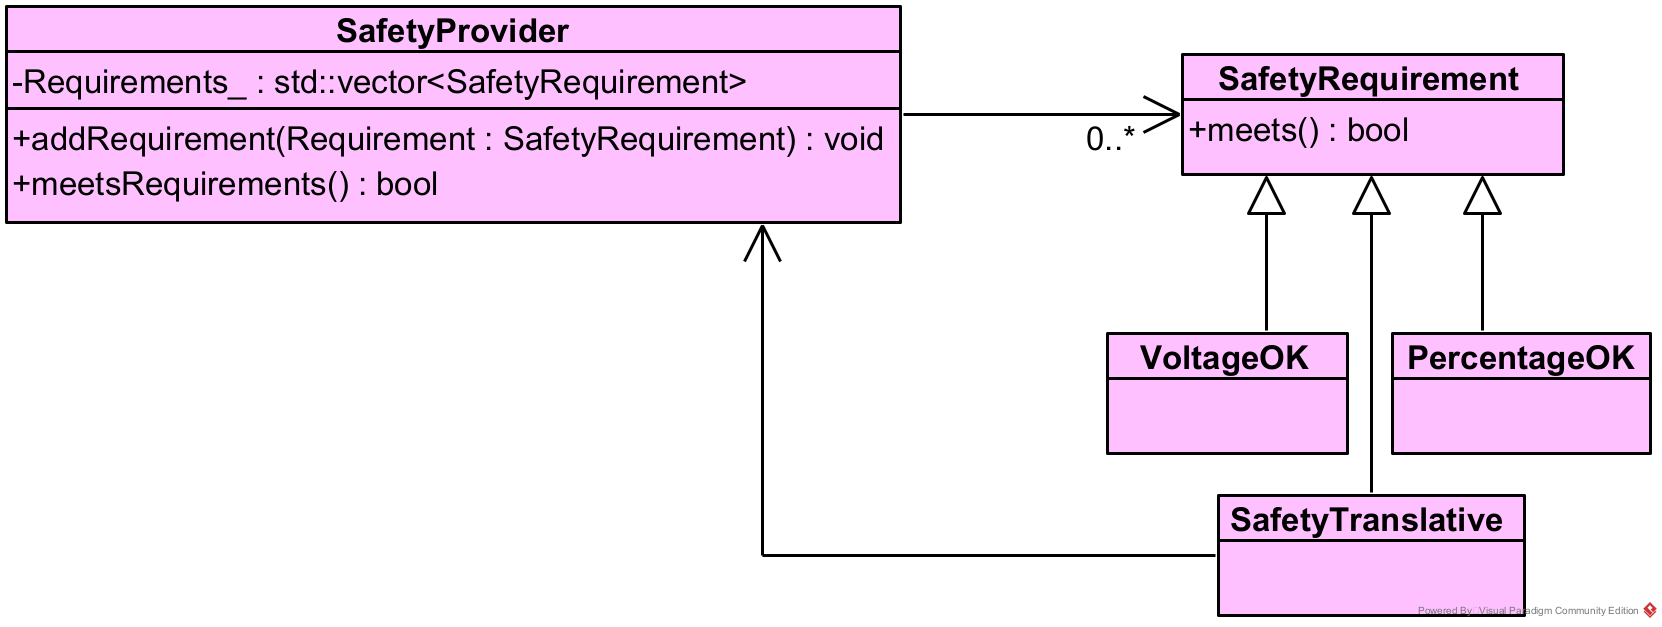
\includegraphics[width=15cm]{Pictures/OpenClose.png}}
\caption{Beispiel-Klassendiagramm für das Open/Close-Principle}
\label{fig:OC}
\end{center}

\vspace{0.25cm}
\href{https://github.com/MaagMich/SWE2\_Project/blob/c5c3674bd201ee306463881cf711bb2ce9229842/Ausarbeitung/Pictures/OpenClose.png}{Image-Link}\\
Die Klassen in \refImgShort{fig:OC} entsprechen der Anordnung der Vorlesungsfolien \glqq Programming Principles\grqq (Seite 18).
\end{figure}


\newSec[PrincSOLIDLisk]{Liskov Substitution Principle}{3}
c++ ist kovariant. Dieses Konzept wurde im Code wie folgt angewandt:

Beispiel:\\
Die in \refCap{MusterBridge} beschriebene Brücke bedient sich der Kovarianz.\\
Es werden Pointer auf Typen in Attributen gespeichert, welche als von diesen Typen abgeleiteten Klassen Instanziiert werden.



\newSec[PrincSOLIDInter]{Interface Segregation Principle}{3}
Wird das \textit{Interface Segregation Principle} umgesetzt, wird der Weg zu \textit{DRY} (siehe \refCap{PrincDRY}) geebnet und eine hohe \textit{Kohäsion} (siehe \refCap{PrincGRASPKohä}) erreicht. Zudem lässt es auf die Umsetzung des \textit{Single Responsibility Principle} (siehe \refCap{PrincSOLIDSingle}) schließen.
Ist ein Projekt ausreichend im Voraus geplant, kann dieses Prinzip deutliche Unterstützung leisten. Für kleinere Projekte, welchen kaum Zeit zugesprochen wird, ist eine entsprechend lange Planung hinderlicht. Es entsteht tendenziell schlechterer Code.

Beispiel im Code:\\
Die \CodeClass{ControlledOutput} setzt sich unmittelbar aus den beiden \textit{virtual} Klassen (\CodeClass{Output} und \CodeClass{Controlable}) zusammen (siehe \refImg{fig:ISP}). Hierdurch wird eine höhere Granularität erreicht.

\begin{figure}[ht!]
\vspace{0.25cm}
\begin{center}
\fbox{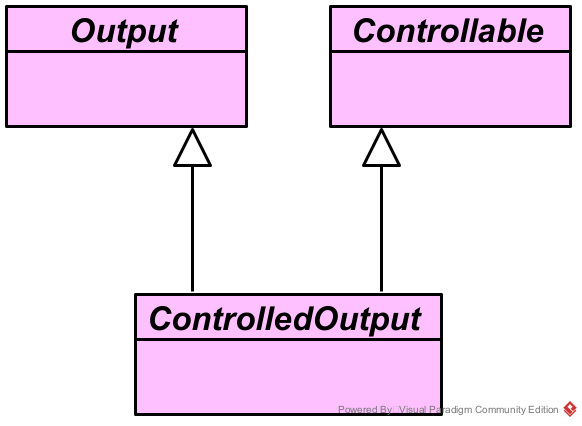
\includegraphics[width=6cm]{Pictures/InterfaceSegregation.png}}
\caption{Beispiel-Klassendiagramm für das Interface Segregation Principle}
\label{fig:ISP}
\end{center}

\vspace{0.25cm}
\href{https://github.com/MaagMich/SWE2\_Project/blob/c5c3674bd201ee306463881cf711bb2ce9229842/Ausarbeitung/Pictures/InterfaceSegregation.png}{Image-Link}
\end{figure}


\newSec[PrincSOLIDDep]{Dependency Inversion Principle}{3}
Eine \textit{Dependency Inversion} ermöglicht eine Veränderung von Programmteilen, ohne den Kern der Anwendung (\textit{Application Layer}) anpassen zu müssen. Ermöglicht wird dies mittels virutellen Klassen\footnotemark[1], welche die im Kern benötigte Grundfunktionalität deklarieren. Die Implementierung findet in der vom Interface erbenden Klasse statt.

Beispiel im Code:\\
\CodeClass{IMUable} besitzt als Attribut einen Pointer auf \CodeClass{PoseBuildable}, welch von der \CodeClass{PoseBuilder} implementiert wird (siehe \refImg{fig:Arch}). Eine Instanz der \CodeClass{PoseBuilder} wird von der Instanz der \CodeClass{MainClass} instanziiert und an die Instanz der \CodeClass{IMUable} übergeben.

